\documentclass[12pt,a4paper]{article}

% Packages standards

\usepackage[utf8]{inputenc}
\usepackage[T1]{fontenc}
\usepackage[francais]{babel}
\usepackage{lmodern}

% Configuration
\def\NomAuteur{Maurice}
\def\PrenomAuteur{Thomas}
\def\Titre{Rapport de projet de quatrième année\\Smart Sensor WiFi}
\def\TitreCourt{Rapport de projet Smart Sensor WiFi}

% Infos du document
% Auteur et tout ça
% Mise en page

\usepackage{hyperref}
\usepackage{fancyhdr}
\usepackage{geometry}
\usepackage{titlesec}
\usepackage{listings}

% Pour include PDF :
% \includepdf[pages=n-m]{fichier.pdf}
\usepackage[final]{pdfpages}

% Urls & figures

\usepackage{url}
\usepackage{graphicx}
\usepackage{wrapfig}

% Configuration de l'article

\hypersetup{
	pdftitle={\Titre}, 	% Titre
	pdfauthor={\PrenomAuteur \NomAuteur}, 	% Auteur
	colorlinks=true,			% Couleur des liens
	linkcolor=black,			% Couleur des liens
	urlcolor=black				% Couleur des liens
}

% Géométrie

\geometry{
	a4paper,
	body={150mm,250mm},
	left=20mm,
	right=20mm,
	top=20mm,
	bottom=20mm,
	headheight=7mm,
	headsep=4mm
}

\pagestyle{empty}

 % Titre du document

\newcommand{\titre}[1]{
						\textbf{
							\LARGE{
								\begin{center}
									#1
								\end{center}
							}
						}
					}

% En-tête du document

\newcommand{\makehead}{
	~~
	\vspace{3cm}
	\titre{\Titre}
	\vspace{3cm}
	\begin{center}
		\PrenomAuteur~\bsc{\NomAuteur} \\
		Benoit \bsc{Maliar} \\~\\
		École Polytechnique Universitaire de Lille \\
		Département IMA \\
		~\\
		\href{mailto:thomas.maurice@polytech-lille.net}{\texttt{Thomas.Maurice@polytech-lille.net}} \\
		\href{mailto:benoit.maliar@polytech-lille.net}{\texttt{Benoit.Maliar@polytech-lille.net}} \\
		~\\
		\today\\
	\end{center}
	\vspace{5cm}
	\begin{center}
		\begin{tabular}{l r}
			
\includegraphics[scale=0.5]{polytech.eps} ~~~~~~~~~ & ~~~~~~~~~ 
\includegraphics[scale=0.5]{ustl.eps} \\
		\end{tabular}
	\end{center}
	
	\newpage
	\renewcommand{\headrulewidth}{0.4pt}
	\renewcommand{\footrulewidth}{0.4pt}
	
	\pagestyle{fancy}
	\fancyhead[L]{\bsc{Maliar - Maurice} IMA4}
	\fancyhead[R]{\TitreCourt}
	\fancyhead[C]{}
	\fancyfoot[C]{}
	
	\tableofcontents
	\newpage
	\pagestyle{fancy}
	\fancyhead[L]{\bsc{Maliar - Maurice} IMA4}
	\fancyhead[R]{\TitreCourt}
	\fancyhead[C]{}
	\fancyfoot[C]{\thepage}
	\setcounter{page}{1}
}

\begin{document}
	\makehead
		
		\setlength{\parskip}{12pt}
		\addcontentsline{toc}{section}{Introduction}
	\section*{Introduction}
		Les projets de quatrième année d'IMA sont l'occasion pour les étudiants
		de mener à bien un projet sur un relativement long terme en partenariat
		avec des industriels ou des laboratoires de recherche. Ils nous permettent
		de mettre en application des connaissances acquises pendant l'année
		et de les perfectionner autour d'un sujet complet, de l'élaboration
		du cahier des charges à une éventuelle réalisation finale.
		\par
		Nous avons donc pu nous pencher sur un problème concret pendant trois
		mois. Le sujet consistait en la réalisation d'un réseau de capteurs
		en wifi pour surveiller de grandes structures et de faire remonter
		des informations d'environnement telles que la température d'une salle,
		son éclairement ou l'éventuelle ouverture ou fermeture d'une porte.
		\par
		De telles données peuvent éventuellement être traitées en amont dans une
		logique d'économie d'énergie, ou tout simplement de surveillance de
		l'état d'un bâtiment.
		

		% !TEX encoding = UTF-8 Unicode
\section{Cahier des charges}
	\par
	Le cahier des charges a été formulé comme il suit : L'objectif du
	projet consiste en la conception et la réalisation de capteurs autonomes
	communiquant en WiFi afin de pouvoir remonter réguliérement des informations
	sur l'état des salles de cours. Les capteurs seront par exemple des détecteurs de
	lumières, de pression, de qualité de l'air, ...
	\par
	La communication sera obligatoirement réalisée en WiFi sur le réseau
	de l'université en respectant les contraintes de sécurité (WPA2, ...).
	\par
	Deux options sont possibles :
	\begin{itemize}
    \item Refaire complètement une carte avec un microcontroleur et une
    puce wifi (comme par exemple les \href{https://www.spark.io/}{spark})
    \item Réaliser un shield pour raspberry pi contenant les différents capteurs. 
	\end{itemize}
	
\section{Présentation de la réalisation}
	\subsection{Présentation de la partie web}
		\par
		La partie Web du projet offre une interface de supervision et de monitoring des capteurs. En effet, nous avons pense qu'il ne suffisait pas de réussir à envoyer des données en Wifi par le biais des capteurs, il fallait aussi pouvoir récupérer et stocker ces informations en vue d'un potentiel traitement. 

	\subsection{Présentation de la partie capteur}
		\subsubsection{Le hardware}
		\par
		A la fin du projet, nous avons réalisé un prototype fonctionnel de ce
		que pourrait être le capteur. Il est important de noter que nous n'avons
		pas cherché à intégrer la solution mais plutôt à la développer en terme
		de fonctionnalités. De ce fait le prototype est assez volumineux mais
		sa taille peut aisément être réduite en utilisant des solutions à base
		de composants CMS notamment ce qui permettrait de réduire de manière
		significative l'encombrement de l'appareil.
		\par
		Le prototype final se compose donc de trois éléments principaux. Le coeur
		du système est réalisé avec un Arduino Uno. Une platine de développement
		sur microcontroleur basée sur un ATmega328P de chez Atmel. C'est dans cet
		Arduino qu'est flashé le programme du capteur. Vient en suite la partie
		qui prend en charge le WiFi, il s'agit d'un shield WiFi de chez GoTronic
		basé sur la puce WizFi210 de WizNet, cette dernière est interfacée avec
		l'Arduino via le port série. Enfin la dernière partie est un protoshield
		sur lequel est placé une breadboard sur laquelle sont enfichés les composants
		avec lesquels l'Arduino peut interagir, à savoir :
		\begin{itemize}
			\item Une photorésistante pour capter la luminosité
			\item Un capteur TMP36 de température
			\item Une RTC (Real Time Clock) DS1302
		\end{itemize}
		Notons que nous avons choisi ces capteurs pour leur facilité d'utilisation,
		mais dans l'absolu rien n'empêche d'utiliser n'importe quel autre capteur
		analogique ou TOR, ni même d'interfacer le système avec des choses plus
		complexes à base de SPI ou d'I$^2$C, étant donné que l'ATmega328P en a
		la possibilité.
		\par
		Le principe de fonctionnement du capteur est très simple. Une fois configuré
		à l'aide de \texttt{configurator} (dont le fonctionnement sera détaillé ci après)
		il vous suffit de déployer le capteur là où vous souhaitez qu'il opère et le
		laisser envoyer des mesures à interval d'une minute. On dispose ainsi
		d'un suivi efficace de l'environnement. Aussitôt que l'appareil est
		mis sous tension il va essayer de se connecter au réseau qui lui a été
		spécifié en configuration et une fois que cela s'est fait proprement il
		va passer en mode interruptif et enverra ses mises à jour toutes les minutes.
		Il faut aussi noter que pendant ce temps là, le capteur écoutera les connexions
		entrantes sur le port 80 et pourra ainsi être reconfiguré par ce biais à l'aide
		d'un set de commandes AT décris et documenté en annexe.
		
		\subsubsection{Le software}
		La partie logicielle du projet est découpée en deux parties. La première
		consiste en le firmware que nous avons chargé dans l'Arduino, et qui est chargé
		de gérer la carte WiFi et les différents capteurs.
		\par
		La seconde partie consiste en un logiciel de configuration écrit spécialement
		pour ce projet, il s'agit de \texttt{configurator}. C'est un script en python
		qui permet via une interface graphique plutôt intuitive de configurer un capteur,
		et ce que ça soit par le port série d'un capteur directement relié au PC en USB
		ou via le réseau en utilisant une socket TCP.

		\section{Détail de la partie web du projet}
\par
Cette partie aura pour but de présenter la partie Web du projet sous un oeil technique. On présentera donc en détail les méthodes utilisées ainsi que les choix techniques qui composent notre projet.
	\subsection{La base de données}
	\par
	La base de données, qui est une base MySQL comme dit précédemment, se compose de 3 tables. De base, nous avions opté pour 2 tables : l'une pour stocker les utilisateurs de la plateforme et leur mot de passe relatif, l'autre pour stocker les capteurs et la mise à jour des données.
	\par
	Ce modèle était valide pour nos tests de début de projet mais s'est montré très limité quand nous avons décidé d'analyser les données des capteurs et spécialement quand nous avons décidé de stocker dans la durée les données. Par exemple, nous avions besoin de plusieurs données d'un même capteur pour dessiner un graphe ou plus simplement comparer différentes mesures.
	Comme nous stockions uniquement la dernière mesure (les informations étaient écrasées à chaque mise à jour), nous ne pouvions stocker plusieurs mesures d'un même capteur. Nous avons donc changé notre implémentation des tables dans la base.
	\par
	Nous aurions pu garder seulement 2 tables, en insérant simplement les nouvelles données dans la table des capteurs au lieu de mettre à jour les champs correspondant. Cette idée n'a pas pu être mise en place car cette table possède un champ 'ID' qui est la clé primaire de la table. Or il aurait fallu avoir plusieurs entrées comportant le même 'ID', ce qui est impossible.
	\par
	C'est donc à ce moment là que la table des capteurs est devenue la table répertoriant la liste des capteurs et une nouvelle table stockant toutes les données des capteurs a été crée.
	\par
	Les relations entre ces différentes tables sont schématisées sur la figure suivante et détaillées ci dessous:
	 \begin{figure}[h]
  		\centering
    		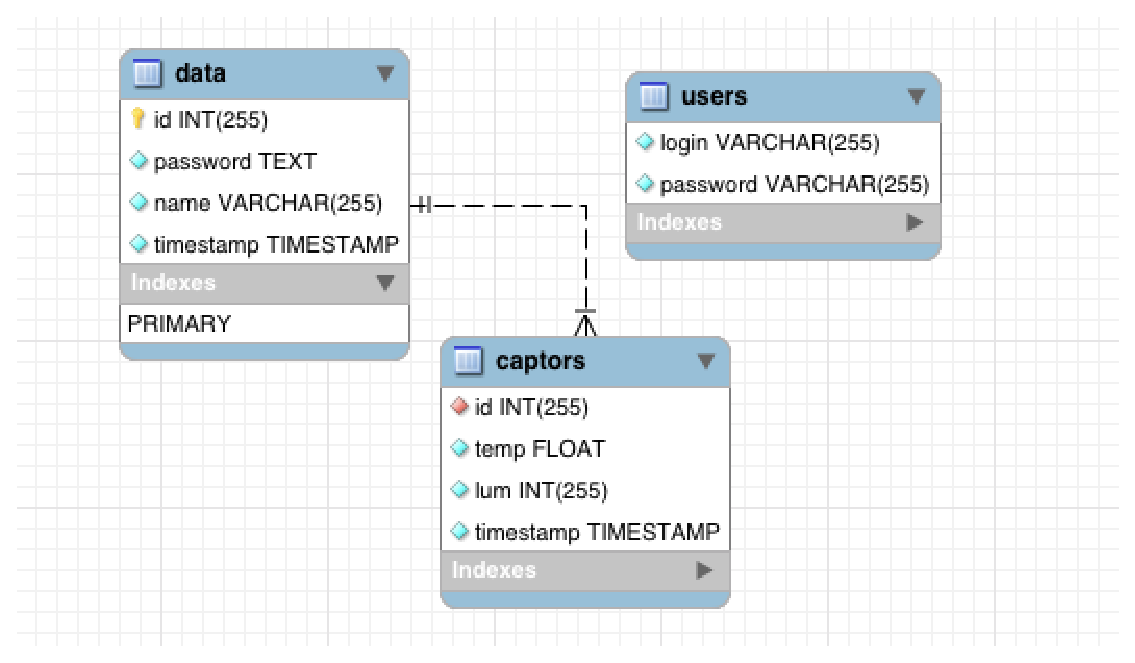
\includegraphics[scale=0.5]{diagramme_tables.eps}
		\caption {diagramme des tables}
	\end{figure}
	\par
	La table 'users' répertorie les différents utilisateurs de la plateforme Web. C'est à travers elle qu'un utilisateur est autorisé à se connecter, sous réserve que son nom et son mot de passe sont corrects.
	\par
	La table 'data' est la table répertoriant les différents capteurs. C'est à travers elle qu'un capteur est autorisé à mettre à jour ses données. Elle stocke aussi la date de dernière mise à jour du de chaque capteur.
	\par
	La table 'captors' est la table stockant les données de chaque capteur. C'est en quelque sorte l'extension de la table 'data'. Chaque champ, défini par son 'ID' ou son 'Name' est relié à une entrée de la table 'data' et complète cette dernière.
	\subsection{La plateforme}
	\par
	Le site se découpe en 4 modules (3 pour un utilisateur lambda) dont un visuel se situe en annexe.
	Pour construire ce site, nous avons utilisé différents langages et outils qui seront développés ci dessous.
	\subsubsection{Les différents modules}
	\par
	Le site Web contient 4 modules différents qui ont chacun une fonction particulière. Le premier est celui qui apparait en premier sur le site. Il autorise la connection à la plateforme. Une fois l'utilisateur connecté, il affiche les 5 dernières mises à jour des capteurs.
	\par
	Le deuxième module permet la recherche d'informations sur un capteur. La recherche s'effectue soit par 'ID' soit par 'Nom'. Une fois le capteur choisi, toutes les données disponibles le concernant s'affiche ansi que deux graphiques des 10 dernières mesures (un pour la température et un pour la luminosité).
	\par
	Le troisième module regroupe l'ajout et la suppression des capteurs. Il est nécessaire de déclarer et autoriser les capteurs en vue de leur mise à jour car si les capteurs ne sont pas répertoriés dans la base, leurs informations ne seront pas prise en compte (permet de sécuriser la mise à jour d'informations au cas où un tierce voudrait compromettre la base de données). Si le capteur n'est plus utilisé, on le supprime de la base à travers cette interface.
	\par
	Le dernier module n'est accessible qu'à l'administrateur de la plateforme. Il regroupe les fonctions d'administration : il permet l'ajout ou la suppression d'un utilisateur, la suppression complète des données des capteurs (en vue d'une remise à zéro) et un panneau de supervision. Ce dernier permet de repérer quels capteurs n'ont pas effectué leur mise à jour (en prenant comme référence la dernière heure). 
	\subsubsection{Le design : Ink}
	\par
	Pour cette plateforme, nous avons voulu faire quelque chose de visuellement propre. C'est donc dans cette optique que nous avons décidé d'utiliser un framework css. Ink est le framework libre qui s'occupe du design de notre site. Il nous a permis de donner un style simple à notre site, une fois maitrisé.
	\par
	La principale difficulté a été de comprendre comment fonctionnait Ink. En effet, en dehors des classes qui lui sont propres, il utilise un système de grille. Chaque morceau du site est découpé et se positionne sur la grille. Ce système structure le site et offre une interface épuré avec de nombreuses possibilité déjà implanté.
	\par
	L'utilisation de Ink se justifie par la qualité visuelle que l'on n'aurait pas pu atteindre par nous même, par manque de temps et certainement de talent graphique.
	\subsubsection{La gestion des données : PHP et Requêtes}
	\par
	L'interaction entre l'utilisateur et le base de données est assurée par PHP. C'est lui qui s'occupe de récupérer, mettre à jour et supprimer les informations demandées ou envoyées par l'utilisateur et le capteur. Il permet aussi d'executer du code en fonction de différents paramètres. C'est lui qui va être le moteur de l'application.
	\par
	Dans un premier temps, il permet d'executer et d'afficher sur la page ce qui est demandé par l'utilisateur, par exemple si l'utilisateur n'a pas encore demandé d'informations sur un capteur, on lui propose de faire un choix entre différents capteurs. Une fois qu'il en a sélectionné un (c'est à dire après l'envoi en POST du choix), PHP récupère cette information et prépare la page pour répondre à la demande de l'utilisateur. Pour illustrer cette fonction, on prend pour exemple le code suivant :
	\\%
	\lstset{language=PHP} 
	\begin{lstlisting}[frame=single]
/*Si on a recu une information d'ID, c'est a dire que l'utilisateur
demande une info sur une ID*/		
if(isset($_POST['id'])){
	//On execute les actions appropriees
}
	\end{lstlisting}
	\par
	La deuxième utilité de PHP est de pouvoir interagir directement avec la BDD. En utilisant PDO, on va se connecter à la base et executer des requêtes qu'on récupérera avec PHP.
	PDO est une méthode orientée objet d'interaction avec différents types de BDD (Mysql, PosgreSQL, etc...) qui est destiné à être la méthode principale à utiliser dans les prochaines versions de PHP. Le choix de PDO se justifie par sa capacité à préparer les requêtes avant de les executer  (on execute les requêtes en fonction de paramètres et non plus statiquement) et par l'importance qu'il prendra dans les versions futures de PHP (il est voué à être la méthode principale de connection, ce qui assure que l'application fonctionnera avec les versions futures).
	\par
	PDO fonctionne de la manière suivante :
	\\%
	\lstset{language=PHP} 
	\begin{lstlisting}[frame=single]
/*On instancie une variable PDO en PHP contenant
toutes les informations de connexion a la base de donnees*/
$bdd = new PDO('mysql:host=hostofthedatabase;dbname=nameofthedb', 
'user', 'password');
/*On prepare la requete avec en option un parametre
represente par "?"*/
$check=$bdd->prepare("SELECT login, password FROM users WHERE
login=?");
/*On execute la requete avec comme parametre "Jesuisunutilisateur"*/
$check->execute(array(Jesuisunutilisateur));
/*On recupere le resultat de la requete dans une variable pour une
utilisation ulterieure*/
$data=$check->fetch();
/*Une fois fini, on ferme proprement la connection a la base de 
donnees*/
$check->closeCursor();
	\end{lstlisting}
		
	\par
	Afin de gérer correctement les échanges d'informations entre le site et la base de données, quatre opérations différentes sont utilisées par PHP/PDO en utilisant le format MySQL :
	\\%
	\begin{itemize}
	\item Insérer des données dans la BDD : 
	\lstset{language=SQL} 
	\begin{lstlisting}[frame=single]
 Ex: INSERT INTO captors(temp,lum,timestamp,id) VALUES(?,?,?,?)
	\end{lstlisting}
	\item Obtenir des données de la BDD : 
	\lstset{language=SQL} 
	\begin{lstlisting}[frame=single]
Ex : SELECT login, password FROM users
	\end{lstlisting}
	\item Mettre à jour des données dans la BDD : 
	\lstset{language=SQL} 
	\begin{lstlisting}[frame=single]
Ex : UPDATE data SET timestamp=? WHERE id=?
	\end{lstlisting}
	\item Supprimer des données dans la BDD : 
	\begin{lstlisting}[frame=single]
Ex : DELETE  captors FROM captors WHERE timestamp  <  ?
	\end{lstlisting}
	\end{itemize}
	\subsubsection{Recup.php}
	\par
	La plus grosse partie du site consiste à faire interagir l'utilisateur avec la base de données. Cependant, il existe une page de site (recup.php) qui n'interagit pas avec l'utilisateur mais avec les capteurs. Celle ci reçoit des informations des capteurs (via POST), vérifie si le capteur a le droit de mettre à jour les données et effectue l'insertion dans la base.
	\par
	Cette page n'a pas seulement l'utilité de mise à jour, elle s'occupe aussi de la conversion des données de température. On s'est aperçu que les mesures brutes des capteurs venant de l'adc devait être multipliées par un coefficient (0,647) pour obtenir une valeur cohérente en température. Cette multiplication n'étant pas faite par l'Arduino (pour le soulager un peu), on a choisi  de donner cette tâche à PHP.
	\par
	En dernier lieu, cette page se charge de nettoyer la table de données des capteurs en supprimer toute entrée datant de la veille via la fonction \href{http://www.php.net/manual/fr/function.date.php}{Date de PHP.}
	\subsubsection{Du dynamisme : Javascript} 
	\par
	Le Javascript sur le site est utilisé pour donner dynamiser l'utilisation du site. Il nous a permis de rediriger automatiquement l'utilisateur et principalement de gérer l'ajout de champ dans les pages d'ajout et de suppression de capteurs.
	En effet, nous l'avons utilisé pour permettre d'effectuer plusieurs actions identiques en une seule fois.
	\par
	Par exemple, quand on veut ajouter en chaine plusieurs capteurs, on aurait pu les ajouter un par mais cela aurait alourdi grandement l'application. La solution est simple, à chaque clic sur un bouton (dans notre cas, un "+"), le javascript insère un nouveau champ sur la page. 
	Cela se traduit par le code suivant : 
	\\%
	\lstset{language=Java} 
	\begin{lstlisting}[frame=single]
// On recupere le cadre ou on va inserer le nouvel element
var div = document.getElementById('champs');

// Fonction qui va creer l'element
function addInput(name,placeholder){
	var input = document.createElement("input");
	input.name = name;
	input.placeholder = placeholder; 
	div.appendChild(input);
}

// On ajoute l'element a la page
	function addField() {
	div.appendChild(document.createElement("br"));
	addInput("name[]","Nom du capteur");
	addInput("password[]","Mot de passe du capteur");
}	
	\end{lstlisting}
	\subsection{Des idées d'amélioration}
	\par
	Plusieurs améliorations peuvent être apportées à la plateforme Web, certaines avaient déjà été pensées au début du projet mais non implantées.
	\par
	En premier lieu, le pattern MVC aurait du être celui de base mais par manque de temps et surtout par sa complexité (principalement avec l'utilisation parallèle d'Ink), il n'a pas été utilisé.
	\par
	Par ailleurs, le site utilise le Javascript mais pourrait l'utiliser plus comme par exemple en rafraichissant la page de recherche d'informations pour permettre d'afficher les dernières informations et le graphique sans devoir recharger manuellement la page.
	\par
	En dernier lieu, on pourrait adapter les différents champs de la base (luminosité, température, etc) ainsi que le code selon les besoins réels (capteur de luminosité, température, pression, etc). On pourrait aussi optimiser le nombre de mesures des graphiques mais cela relève plus de l'optimisation que de l'amélioration.
		\section{Détail de la conception de la partie microcontrôleur du projet}
	\subsection{Le capteur}
		Lors de la réalisation du capteur il a fallu en premier lieu se fixer
		des objectifs à atteindre, afin d'être sur d'aller dans une direction
		cohérente tout a long du projet. De  ce fait nous avons choisi d'opter pour
		la réalisation d'un prototype fonctionnel et relativement simple au début.
		Par relativement simple, nous entendions capable de lire un ou deux capteurs
		analogiques simples à mettre en place de manière à nous focaliser sur
		l'interfaçage du dispositif avec un serveur de données. Nous nous sommes
		donc d'avantage focalisés sur une approche plus logicielle du projet en
		écartant volontairement, par manque de temps, des considérations annexes
		comme la gestion de l'énergie ou la mise en place immédiate de capteurs
		très complexes. Le but était réellement de fournir une base saine sur laquelle
		il serait facile de se baser à l'avenir.
		
		\subsubsection{La partie électronique}
		
		La partie électronique est la plus simple de l'appareil c'est donc celle
		là qui sera abordée en premier. Elle se compose simplement d'une photo résistance
		montée en pull up sur la patte analogique 1 de l'Arduino et d'un capteur de
		température câblé sur la patte analogique 2. Nous avons également câblé un bouton de
		mise à jour (dont l'utilité sera détaillée plus tard) sur la patte PD2
		ainsi que la real time clock sur trois pattes numériques de manière à pouvoir
		échanger des données. Tout ces composants ont été positionnés sur une breadboard
		de manière à ce que nous puissions facilement en modifier l'arrangement au fur et a mesure
		que nos besoins évoluaient dans le projet.
		\par
		Nous n'avons malheureusement pas eu le temps de réaliser de carte
		pour fixer ce design. Et il n'aurait pas été pertinent de le faire dans la mesure
		ou la conception, le routage et la fabrication d'une carte sont des activités pour
		le moins chronophages et qu'il a effectivement été plus productif pour nous de nous
		concentrer sur l'ajout de nouvelles fonctionalités au capteur. Cependant
		nous avons édités des PCB et des schémas électroniques disponibles en
		annexe qui permettent de réaliser une telle carte.
		
		\subsubsection{Conception du firmware de l'Arduino}
		La conception du firmware de l'arduino s'est découpée en plusieurs étapes.
		Pour commencer nous avons séparé les différentes fonctionnalités que nous
		souhaitions. D'un point de vue organisation cela s'est traduit par un fractionnement
		du code en plusieurs fichiers, chacun regroupant les fonctions relatives à un
		domaine, par exemple la gestion du port série, des CAN, de l'EEPROM et autre.
		\par
		Ensuite, une fois que la séparation logique des fonctionalités a été effectuée
		nous avons commencé à les développer une à une, en lançant à chaque fois une
		série de tests sur ce que nous avions créé, de manière à nous assurer que tout
		était bien conforme à ce que nous attendions. De cette manière nous pouvions
		réutiliser sans crainte du code que nous avions précédemment écrit puisqu'il
		avait été validé par une batterie de tests.
		\par
		Une attention toute particulière a été portée à la doc. En effet si nous
		souhaitons que le projet puisse être repris les années suivantes il
		est indispensable de fournir une documentation valable, fiable et complète
		de manière à ce que n'importe qui ou presque soit en mesure de comprendre
		ce qui a déjà été réalisé de manière logicielle. Pour ce faire nous avont eu
		recours au système de documentation in-code Doxygen, qui grâce à un
		système de commentaires au formattage particulier permet de générer automatiquement
		une belle documentation HTML. Cette documentation navigable est facile à utiliser, avec outils
		de recherche intégré et liens entre les différentes fonctions documentées.
		Si vous souhaitez construire la documentation du programme rendez vous dans
		le répertoire Arduino et tapez simplement \texttt{doxygen} un dossier contenant
		le nécessaire sera généré pour vous !
		\par
		La seconde partie du projet, qui n'est au final même pas utilisée dans le prototype
		actuel, a été la réalisation d'un driver pour la real time clock de Maxim DS1302. En
		effet, nous somme parti du constat que le fonctionnement du WiFi pouvait être parfois
		assez instable, et que de ce fait il serait appréciable que le capteur puisse se comporter
		comme une sorte de datalogger dans le cas où il serait dans l'incapacité momentanée de communiquer
		avec le serveur de donnée, que cela soit a cause du wifi ou d'un autre problème d'ailleurs.
		Pour cela nous avions pensé le coupler avec une flash (voir les schémas en annexe). Cela dit
		comme le composant n'était disponible qu'en format SOIC8 et que nous n'avons pas réalisé la carte
		il nous a été impossible de l'intégrer correctement. Une amélioration possible et très facile à
		mettre en oeuvre pour le projet serait donc l'intégration de cette flash et l'utilisation
		de la RTC pour soumettre en différé des données de mesures qui n'aurais pas pu être
		transmises à temps.
		\par
		La troisième partie du projet a été consacrée à faire en sorte que la configuration du capteur
		soit persistante entre les reboots. Durant les phases de développement nous ne nous étions pas
		vraiment occupé de cela mais dès que le programme est devenu plus compliqué il est devenu
		essentiel de stocker certains paramètres (d'identifications notamment) autrement qu'en dur
		dans le code. Il a donc fallu ajouter un module de gestion de l'EEPROM. La structure suivante a donc
		été choisie pour stocker des données :
		\begin{itemize}
			\item L'EEPROM est découpée en différents secteur de taille fixé à la compilation
			\item Chaque secteur contient un octet de taille et $N$ octets de données ($N < 255$)
			\item Chaque secteur est uniquement défini par sa position en mémoire
		\end{itemize}
		
		Cette solution présente l'avantage d'être très simple à mettre en place d'un point de vue
		logiciel, ce système souffre cependant d'un gros problème qui est que l'on ne peut
		pas connaitre de manière dynamique la taille maximale des données que l'on peut ranger
		dans un segment. Ce qui implique que le programmeur fasse très attention aux données qu'il
		manipule, de manière à ne pas provoquer de débordement sur un autre segment. Ceci dit,
		ce problème n'est pas vraiment critique puisqu'une simple réécriture de la configuration
		rétablira tout correctement. Ceci fait également partie des améliorations possibles
		du projet.
		
		\par
		La quatrième partie du projet a sans aucun doute été la plus difficile à réaliser. En
		effet après s'être occupé des briques élémentaire qui compose le capteur (communiquer
		en série, lire des capteurs analogiques, lire la RTC). Il a fallu regrouper tout ça
		ensemble et l'envoyer sur internet. Pour se faire, il a d'abord fallu comprendre comment
		fonctionnait la carte WiFi. La datasheet n'étant pas toujours très claire, ni très complète
		il a d'abord fallu passer par une phase \og{} d'exploration \fg{} de la carte via le port
		série, de manière à comprendre précisément ce qu'elle attendais de nous en terme de commandes.
		La carte se configurait finalement par un set de commandes AT via le port série et malgré
		les quelques imprécisions de la datasheet nous avons finalement été capables de nous identifier
		sur un réseau spécialement créé pour l'occasion.
		
		\par
		A partir de là a été développé une petite bibliothèque qui intègre les fonctions réseau de base,
		à savoir s'identifier sur un réseau avec des paramètres donnés, soumettre des requêtes HTTP et
		vérifier le retour des commandes AT de manière à réitérer plusieurs fois une tentative de connexion
		qui aurait échouée.
		
		\subsubsection{Interaction du capteur avec les internets}
		
		\subsubsection{Principales difficultés rencontrées}
		
	\subsection{Configurator.py}

		\addcontentsline{toc}{section}{Conclusion}
	\section*{Conclusion}
		Texte de conclusion

		~~
\vspace{10cm}

\begin{center}
\Huge{Annexes}
\end{center}
\newpage

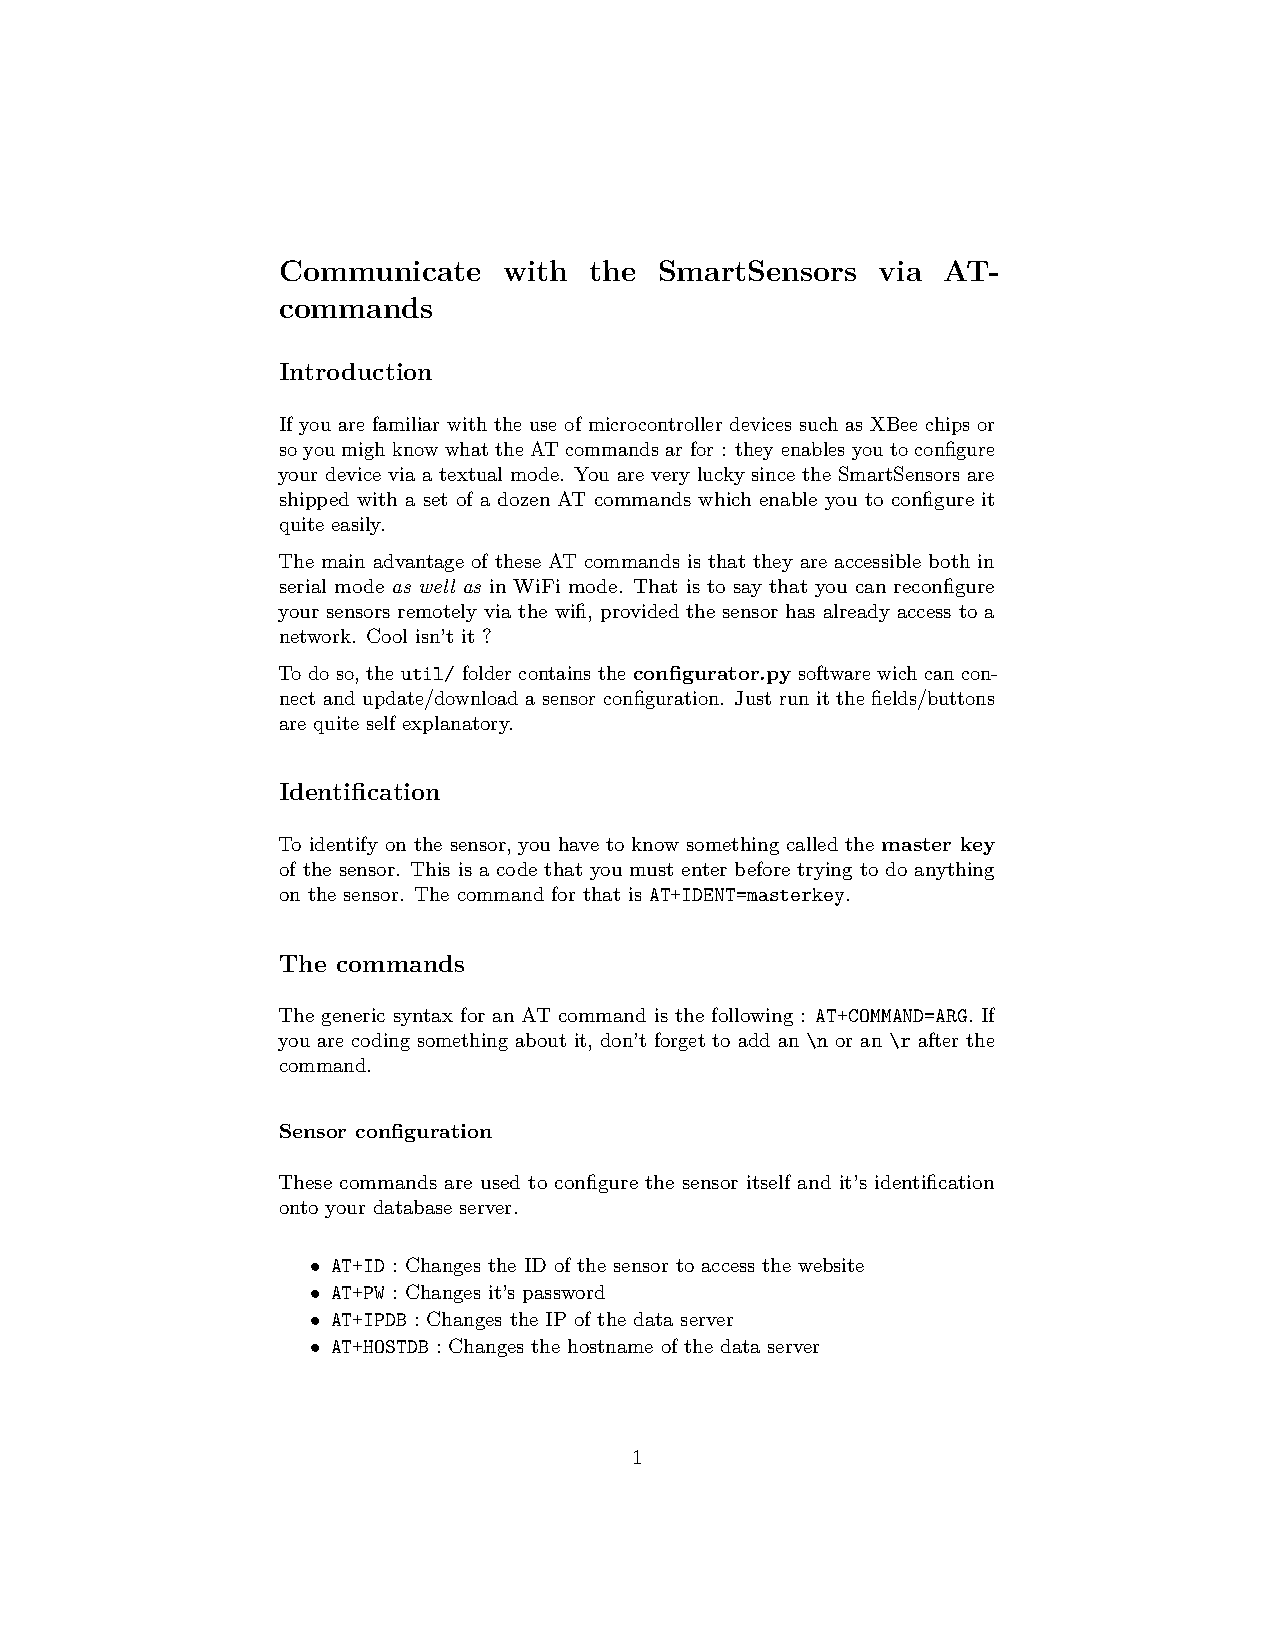
\includepdf[pages={1-}]{SensorATCommands.pdf}
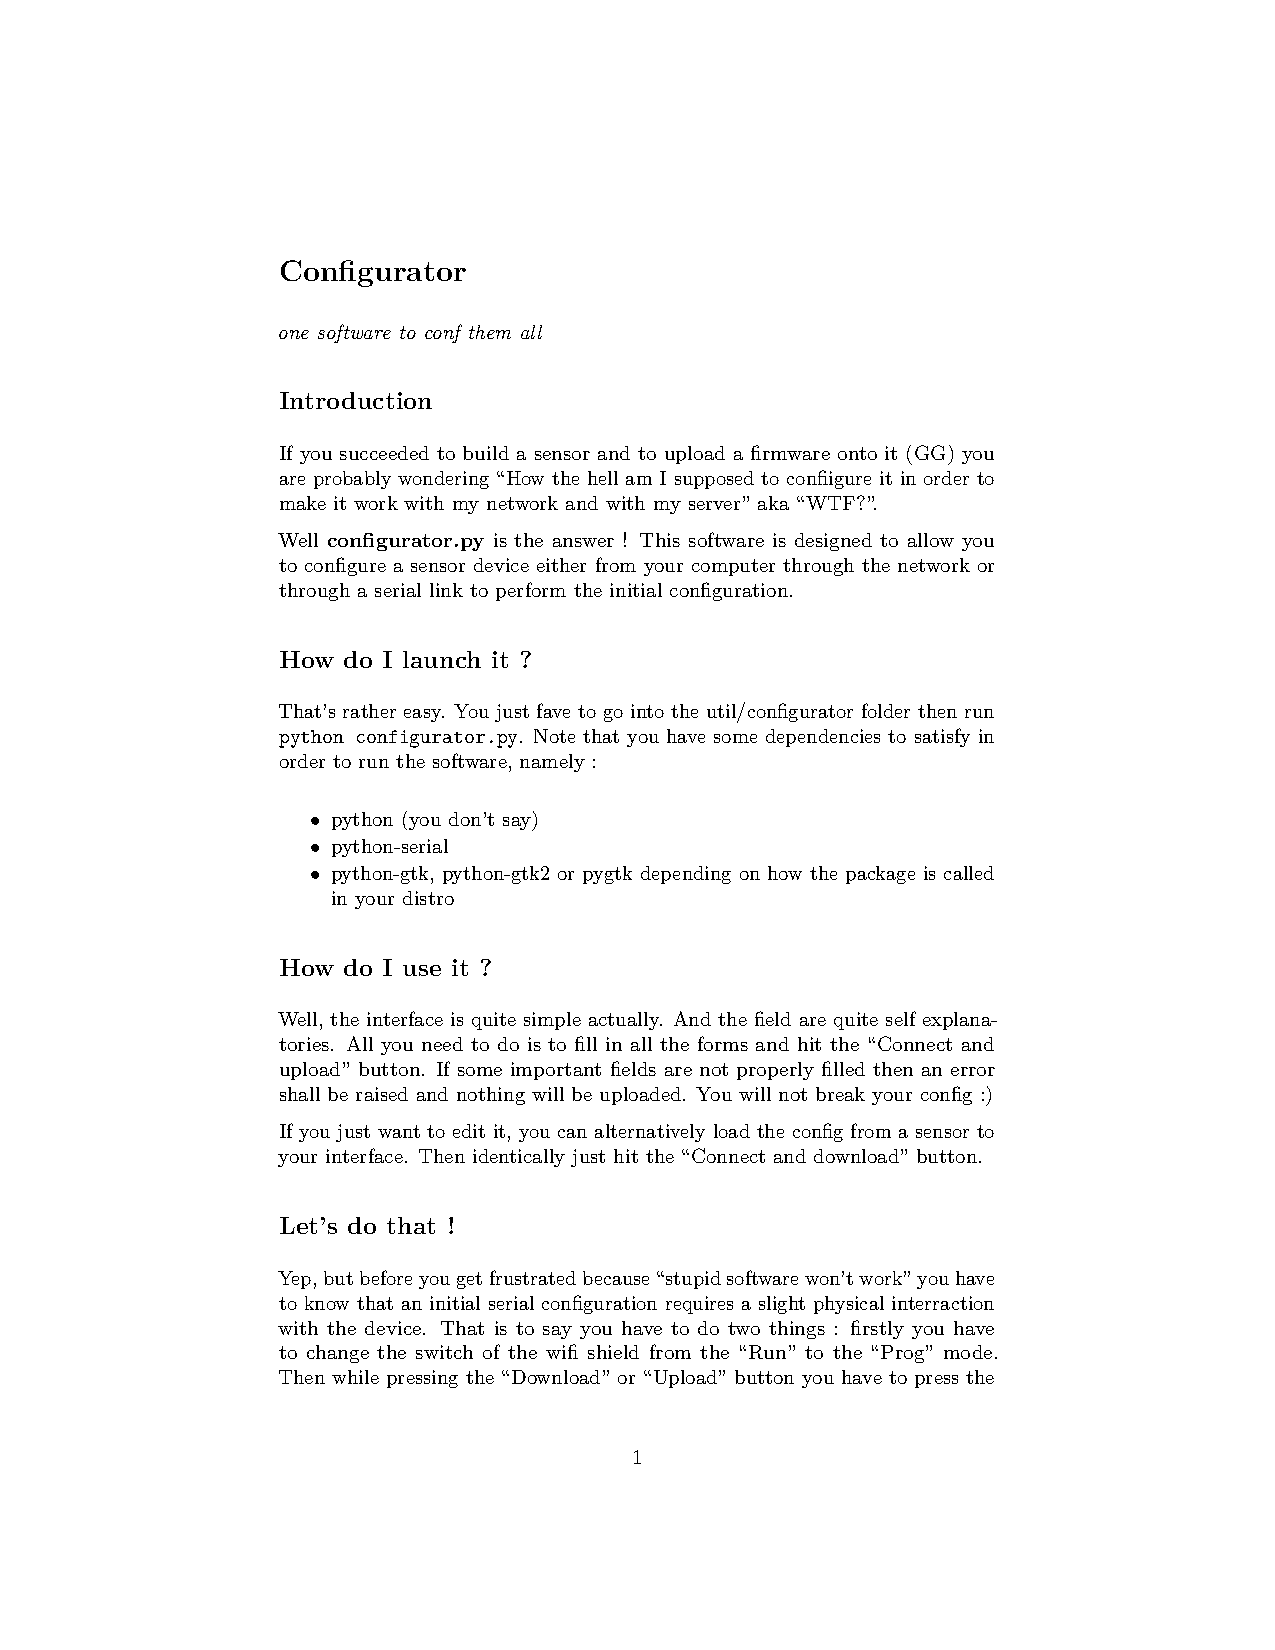
\includepdf[pages={1-}]{useConfigurator.pdf}
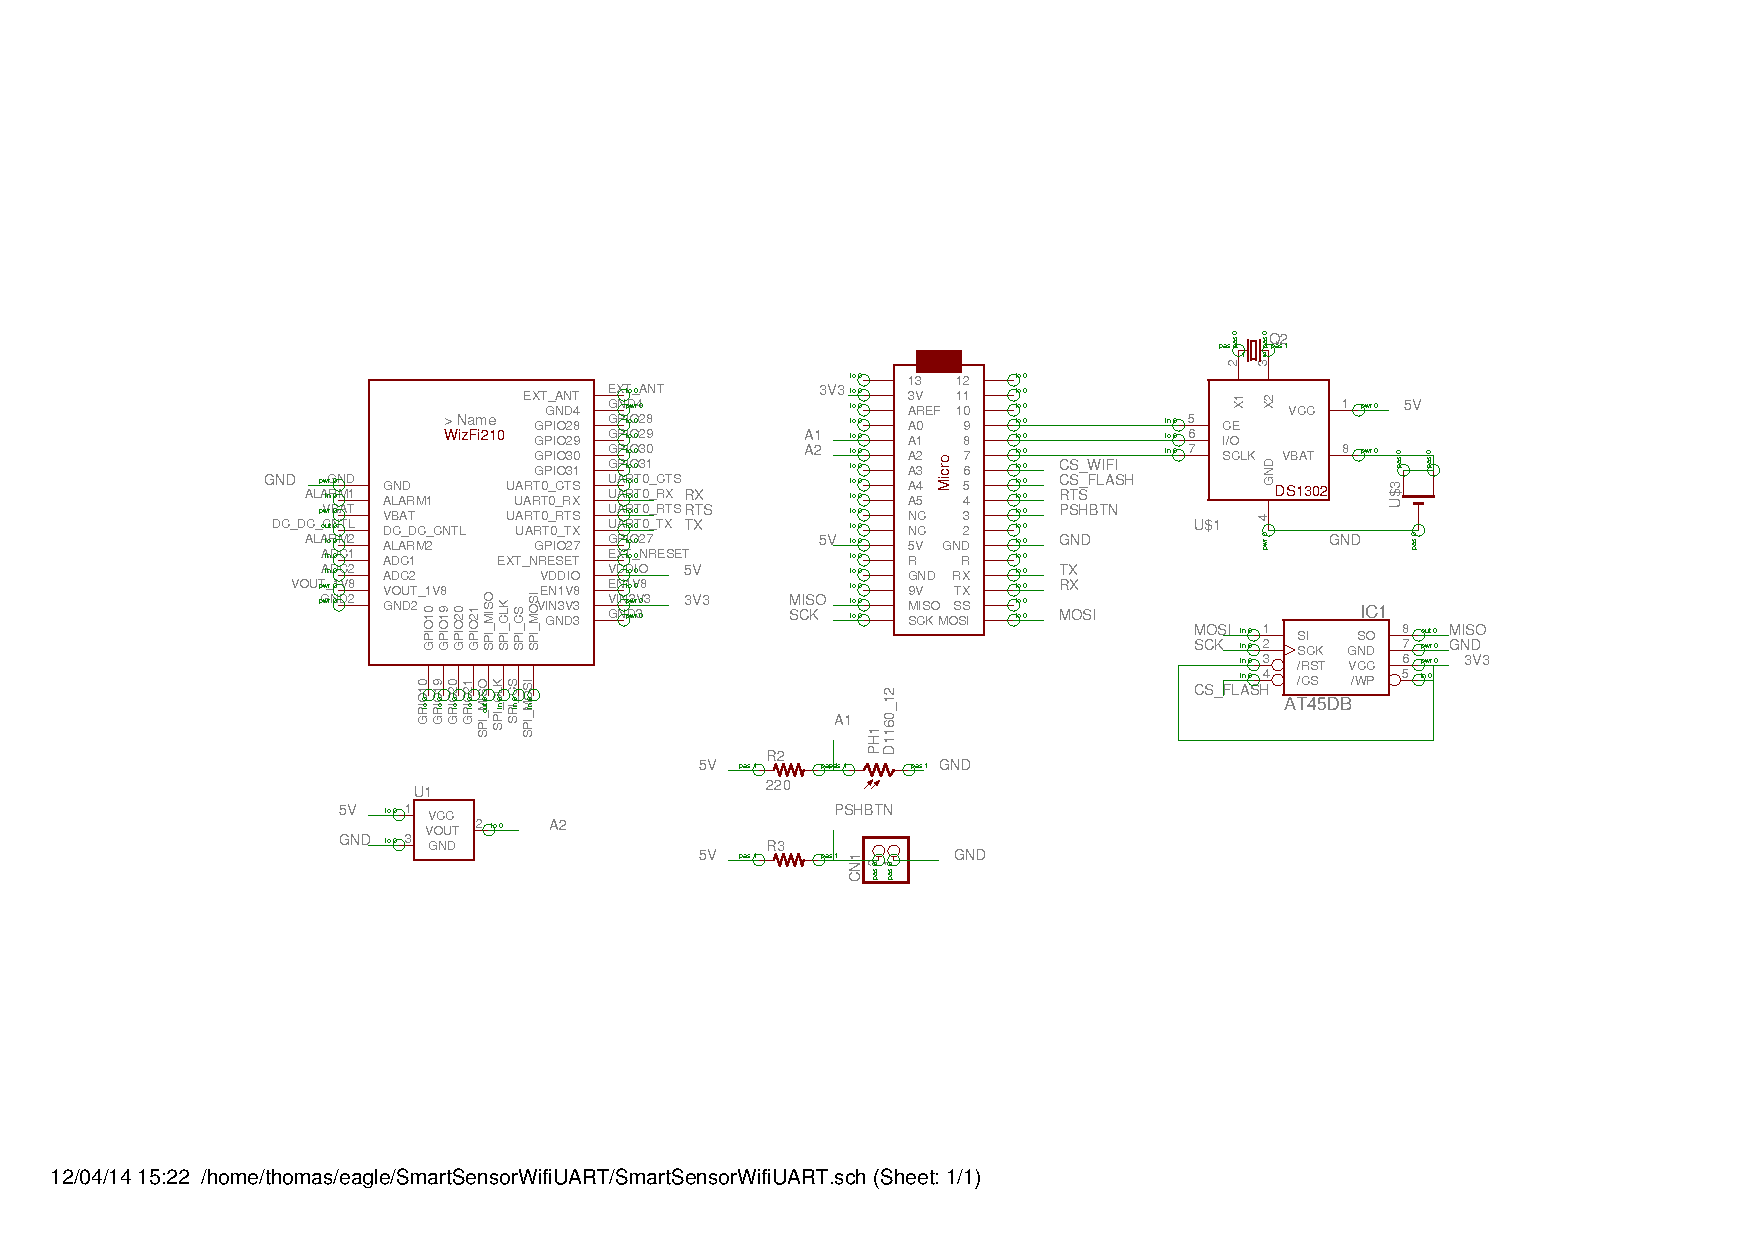
\includepdf[pages={1-}]{SmartSensorWifiUART.pdf}
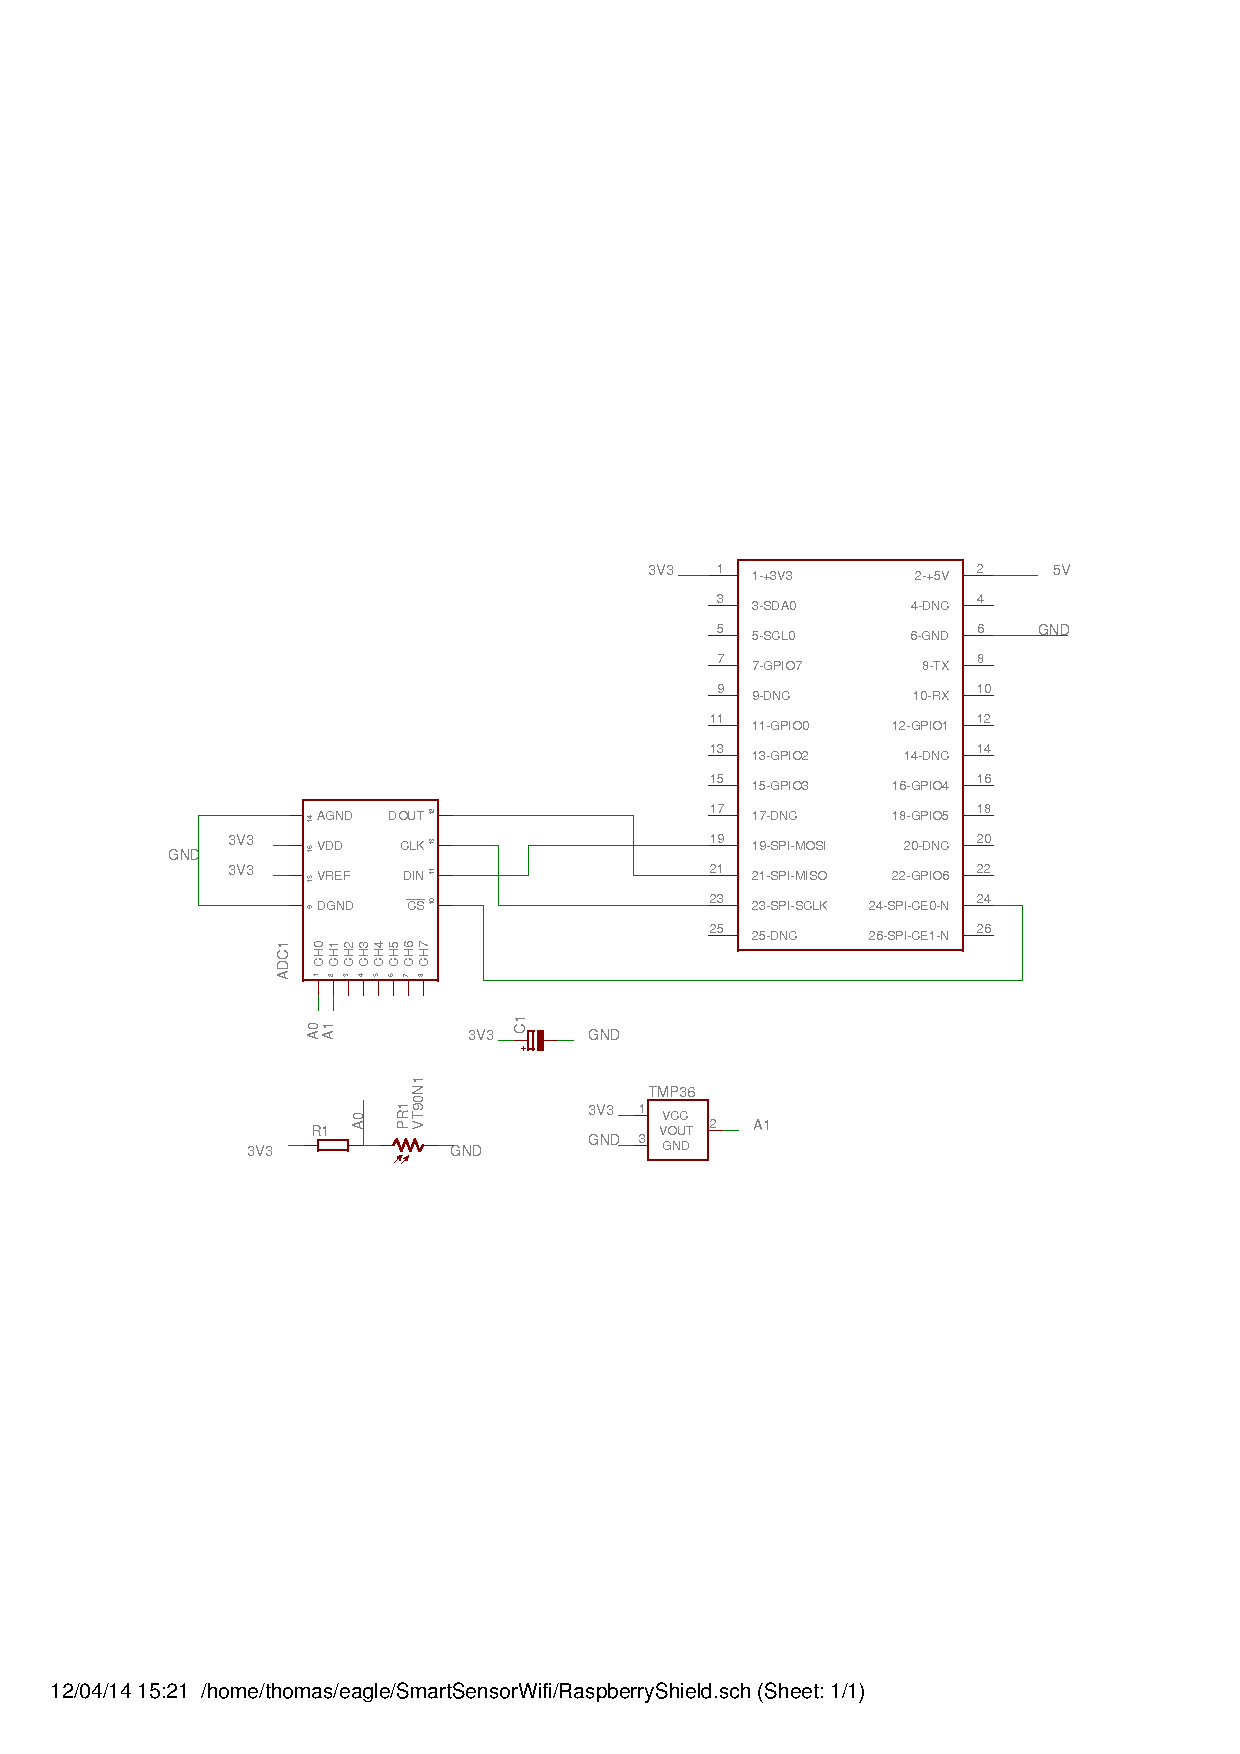
\includepdf[pages={1-}]{RaspberryShield.pdf}

		
\end{document}
